\documentclass{elsarticle}

% Standalone Supplementary Information for the Scientific Data submission.
% Shares its body (supplementary_sections.tex) with manuscript.tex, which
% embeds the same sections as an appendix in the combined working PDF.
% Compile with: latexmk -pdf supplementary.tex

\providecommand{\ZenodoDoi}{10.5281/zenodo.18961227}
\providecommand{\ZenodoUrl}{https://doi.org/10.5281/zenodo.18961227}

\usepackage[utf8]{inputenc}
\usepackage[margin=2.5cm]{geometry}
\usepackage{graphicx}
\usepackage{booktabs}
\PassOptionsToPackage{hyphens}{url}\usepackage{hyperref}
\usepackage{siunitx}
\usepackage{xcolor}
\usepackage{longtable}
\usepackage{multirow}
\usepackage{array}
\usepackage{float}
\usepackage{placeins}
\usepackage{enumitem}
\usepackage{caption}
\usepackage{wrapfig}
\usepackage{amssymb}
\usepackage{pdflscape}

% Allow line breaks after underscores in long \texttt{} filenames.
\renewcommand{\_}{\textunderscore\allowbreak}

\makeatletter
\pdfstringdefDisableCommands{%
  \def\corref#1{}%
  \def\cnotenum{}%
  \def\@corref#1{}%
}
\makeatother

% Auto-generated statistics macros (from paper_stats.json)
% Auto-generated LaTeX macros
% Generated by: python paper_data/code/s06_write_paper_macros.py
% DO NOT EDIT MANUALLY - regenerate from source data
% === City Counts ===
\newcommand{\NCitiesTotal}{626}
\newcommand{\NCountries}{28}
\newcommand{\NRefCities}{116}
\newcommand{\NRefCitiesFr}{73}
\newcommand{\NRefCitiesNl}{43}
\newcommand{\NNonRefCities}{510}

% === Data Coverage ===
\newcommand{\NCitiesLowHeight}{94}
\newcommand{\NCitiesNoHeight}{20}
\newcommand{\NCitiesWithHeightsRaster}{611}
\newcommand{\BldgHeightsAgeYears}{14}
\newcommand{\MedianHeightCoverage}{71}
\newcommand{\MedianBlockHundredCoverage}{74}
\newcommand{\NCitiesNoBlocks}{24}
\newcommand{\NCitiesNoEmployment}{185}

% === Dataset Size ===
\newcommand{\DatasetTotalCompressedGB}{35}
\newcommand{\DatasetMinMB}{3.5}
\newcommand{\DatasetMaxGB}{1.2}
\newcommand{\DatasetMeanMB}{56}

% === POI Validation Thresholds ===
\newcommand{\PoiNearDistGoodM}{800}
\newcommand{\PoiNearDistOtherM}{800}
\newcommand{\PoiNearDistAccomM}{1200}

% === Displacement Stats ===


% Consistent table column types
\newcolumntype{L}[1]{>{\raggedright\arraybackslash}p{#1}}
\newcolumntype{C}[1]{>{\centering\arraybackslash}p{#1}}
\newcolumntype{R}[1]{>{\raggedleft\arraybackslash}p{#1}}

\journal{Scientific Data}

\begin{document}

\begin{frontmatter}

  \title{Supplementary Information for: SOAR-EU: A Scalable, Open, Automatable, and Reproducible European Urban Dataset}

  \author[spacesyntax]{Gareth Simons\corref{cor1}}
  \ead{gareth.simons@ucl.ac.uk}
  \cortext[cor1]{Corresponding author}

  \author[spacesyntax]{Kayvan Karimi}
  \author[spacesyntax]{Sepehr Zhand}

  \affiliation[spacesyntax]{organization={Space Syntax Laboratory, UCL Bartlett School of Architecture},
    addressline={22 Gordon Street},
    city={London},
    country={United Kingdom}
  }

\end{frontmatter}

\appendix
\renewcommand{\thesection}{S\arabic{section}}
% Sequential S-numbering for supplementary floats, matching the combined
% manuscript's appendix so main-text cross-references resolve in both documents.
\setcounter{figure}{0}
\setcounter{table}{0}
\renewcommand{\thefigure}{S\arabic{figure}}
\renewcommand{\thetable}{S\arabic{table}}

% Supplementary Information sections (S1-S5), shared between
% manuscript.tex (combined working PDF) and supplementary.tex
% (standalone SI for Scientific Data submission).
\section{Complete Streets Layer Schema}
\label{sec:streets-schema}

The streets layer contains street segments with computed metrics. Distance thresholds vary by metric type: centrality at 400\,m, 800\,m, 1200\,m, 1600\,m, 4800\,m, 9600\,m; accessibility at 200\,m, 400\,m, 800\,m, 1200\,m, 1600\,m; morphology at 200\,m, 400\,m; green space proximity at 1600\,m; green area aggregation at 200\,m, 400\,m, 800\,m. Table~\ref{tab:complete_streets} provides the complete attribute schema.

\begin{landscape}
  \scriptsize
  \begin{longtable}{@{}L{7cm}L{2cm}L{8cm}L{3cm}@{}}
    \caption{Complete streets layer attribute schema. Suffix \texttt{\_DDD} indicates distance threshold in metres. Source abbreviations: Ovt net = Overture street networks; Ovt POI = Overture POIs; Ovt infra = Overture infrastructure; Ovt bldg = Overture building footprints; UA = Copernicus Urban Atlas; STL = Copernicus Street Tree Layer; CHM = Copernicus Height Model.} \label{tab:complete_streets} \\
    \toprule
    \textbf{Attribute} & \textbf{Type} & \textbf{Description} & \textbf{Source} \\
    \midrule
    \endfirsthead

    \multicolumn{4}{c}%
    {{\tablename\ \thetable{} -- continued from previous page}} \\
    \toprule
    \textbf{Attribute} & \textbf{Type} & \textbf{Description} & \textbf{Source} \\
    \midrule
    \endhead

    \midrule
    \multicolumn{4}{r}{{Continued on next page}} \\
    \endfoot

    \bottomrule
    \endlastfoot

    \multicolumn{4}{l}{\textbf{Geometry and Identifiers}} \\
    \midrule
    \texttt{geometry} & LineString & Street segment geometry (EPSG:3035) & Ovt net \\
    \texttt{ns\_node\_idx} & Integer & Internal network node index & Ovt net \\
    \texttt{x} & Float & Segment midpoint X coordinate (EPSG:3035) & Ovt net \\
    \texttt{y} & Float & Segment midpoint Y coordinate (EPSG:3035) & Ovt net \\
    \texttt{seg\_length} & Float & Street segment length (m) & Ovt net \\
    \midrule

    \multicolumn{4}{l}{\textbf{Network Centrality (Segment-Based, DDD = 400, 800, 1200, 1600, 4800, 9600)}} \\
    \midrule
    \texttt{cc\_beta\_DDD} & Float & Beta-weighted closeness (gravity index with exponential decay) & Ovt net \\
    \texttt{cc\_cycles\_DDD} & Float & Cycle count within threshold & Ovt net \\
    \texttt{cc\_density\_DDD} & Float & Street segment density within threshold & Ovt net \\
    \texttt{cc\_farness\_DDD} & Float & Total network distance to reachable segments & Ovt net \\
    \texttt{cc\_harmonic\_DDD} & Float & Harmonic closeness (sum of inverse distances) & Ovt net \\
    \texttt{cc\_hillier\_DDD} & Float & Hillier-type closeness (node count / avg distance) & Ovt net \\
    \texttt{cc\_betweenness\_DDD} & Float & Segment betweenness centrality & Ovt net \\
    \texttt{cc\_betweenness\_beta\_DDD} & Float & Beta-weighted betweenness centrality & Ovt net \\
    \midrule

    \multicolumn{4}{l}{\textbf{Accessibility -- POI Counts (DDD = 200, 400, 800, 1200, 1600)}} \\
    \midrule
    \texttt{cc\_accommodation\_DDD\_nw} & Integer & Unweighted count of accommodation POIs & Ovt POI \\
    \texttt{cc\_accommodation\_DDD\_wt} & Float & Distance-weighted count of accommodation POIs & Ovt POI \\
    \texttt{cc\_accommodation\_nearest\_max\_1600} & Float & Distance to nearest accommodation POI (m) & Ovt POI \\
    \texttt{cc\_active\_life\_DDD\_nw/wt} & Float & Active life POI counts (unweighted/weighted) & Ovt POI \\
    \texttt{cc\_arts\_and\_entertainment\_DDD\_nw/wt} & Float & Arts and entertainment POI counts & Ovt POI \\
    \texttt{cc\_attractions\_and\_activities\_DDD\_nw/wt} & Float & Attractions and activities POI counts & Ovt POI \\
    \texttt{cc\_business\_and\_services\_DDD\_nw/wt} & Float & Business and services POI counts & Ovt POI \\
    \texttt{cc\_eat\_and\_drink\_DDD\_nw/wt} & Float & Eat and drink POI counts & Ovt POI \\
    \texttt{cc\_education\_DDD\_nw/wt} & Float & Education POI counts & Ovt POI \\
    \texttt{cc\_health\_and\_medical\_DDD\_nw/wt} & Float & Health and medical POI counts & Ovt POI \\
    \texttt{cc\_public\_services\_DDD\_nw/wt} & Float & Public services POI counts & Ovt POI \\
    \texttt{cc\_religious\_DDD\_nw/wt} & Float & Religious POI counts & Ovt POI \\
    \texttt{cc\_retail\_DDD\_nw/wt} & Float & Retail POI counts & Ovt POI \\
    \texttt{cc\_\{category\}\_nearest\_max\_1600} & Float & Distance to nearest POI in category (m) & Ovt POI \\
    \midrule

    \multicolumn{4}{l}{\textbf{Infrastructure Accessibility (DDD = 200, 400, 800, 1200, 1600)}} \\
    \midrule
    \texttt{cc\_transport\_DDD\_nw/wt} & Float & Transport stops/stations counts & Ovt infra \\
    \texttt{cc\_street\_furn\_DDD\_nw/wt} & Float & Street furniture counts (benches, fountains) & Ovt infra \\
    \texttt{cc\_parking\_DDD\_nw/wt} & Float & Parking facility counts & Ovt infra \\
    \midrule

    \multicolumn{4}{l}{\textbf{Mixed-Use Diversity Indices (DDD = 200, 400, 800, 1200, 1600)}} \\
    \midrule
    \texttt{cc\_hill\_q0\_DDD\_nw} & Float & Hill diversity (q=0, richness) unweighted & Ovt POI \\
    \texttt{cc\_hill\_q0\_DDD\_wt} & Float & Hill diversity (q=0, richness) distance-weighted & Ovt POI \\
    \texttt{cc\_hill\_q1\_DDD\_nw} & Float & Hill diversity (q=1, exp Shannon) unweighted & Ovt POI \\
    \texttt{cc\_hill\_q1\_DDD\_wt} & Float & Hill diversity (q=1, exp Shannon) distance-weighted & Ovt POI \\
    \texttt{cc\_hill\_q2\_DDD\_nw} & Float & Hill diversity (q=2, inv Simpson) unweighted & Ovt POI \\
    \texttt{cc\_hill\_q2\_DDD\_wt} & Float & Hill diversity (q=2, inv Simpson) distance-weighted & Ovt POI \\
    \midrule

    \multicolumn{4}{l}{\textbf{Building Morphology (DDD = 200, 400; stat = median, mad; suf = nw, wt)}} \\
    \midrule
    \texttt{cc\_area\_\{stat\}\_DDD\_\{suf\}} & Float & Building area statistics (m\textsuperscript{2}) & Ovt bldg \\
    \texttt{cc\_area\_sum\_DDD\_\{suf\}} & Float & Total building area within threshold (m\textsuperscript{2}) & Ovt bldg \\
    \texttt{cc\_perimeter\_\{stat\}\_DDD\_\{suf\}} & Float & Building perimeter statistics (m) & Ovt bldg \\
    \texttt{cc\_compactness\_\{stat\}\_DDD\_\{suf\}} & Float & Circular compactness ($A / A_{\text{encl}}$) & Ovt bldg \\
    \texttt{cc\_orientation\_\{stat\}\_DDD\_\{suf\}} & Float & Orientation angle (degrees) & Ovt bldg \\
    \texttt{cc\_mean\_height\_\{stat\}\_DDD\_\{suf\}} & Float & Building height (m) & CHM \\
    \texttt{cc\_volume\_\{stat\}\_DDD\_\{suf\}} & Float & Building volume (m\textsuperscript{3}) & Ovt bldg + CHM \\
    \texttt{cc\_volume\_sum\_DDD\_\{suf\}} & Float & Total building volume within threshold (m\textsuperscript{3}) & Ovt bldg + CHM \\
    \texttt{cc\_form\_factor\_\{stat\}\_DDD\_\{suf\}} & Float & Form factor ($S / V^{2/3}$, $S = Ph + A$) & Ovt bldg + CHM \\
    \texttt{cc\_corners\_\{stat\}\_DDD\_\{suf\}} & Float & Corner count & Ovt bldg \\
    \texttt{cc\_shape\_index\_\{stat\}\_DDD\_\{suf\}} & Float & Shape index & Ovt bldg \\
    \texttt{cc\_shared\_wall\_ratio\_\{stat\}\_DDD\_\{suf\}} & Float & Shared wall ratio (fraction of perimeter) & Ovt bldg \\
    \texttt{cc\_fractal\_dimension\_\{stat\}\_DDD\_\{suf\}} & Float & Fractal dimension & Ovt bldg \\
    \texttt{cc\_building\_DDD\_nw/wt} & Float & Building count (unweighted/weighted) & Ovt bldg \\
    \texttt{frontage\_max} & Float & Bilateral street-frontage ratio (0--1); max of left/right building edge coverage within 35\,m corridor & Ovt bldg \\
    \texttt{frontage\_avg} & Float & Mean of left and right frontage coverage & Ovt bldg \\
    \texttt{frontage\_left} & Float & Left-side frontage coverage & Ovt bldg \\
    \texttt{frontage\_right} & Float & Right-side frontage coverage & Ovt bldg \\
    \texttt{frontage\_edges\_left} & Integer & Count of building edges contributing to left-side coverage & Ovt bldg \\
    \texttt{frontage\_edges\_right} & Integer & Count of building edges contributing to right-side coverage & Ovt bldg \\
    \midrule

    \multicolumn{4}{l}{\textbf{Green Space Proximity (DDD = 200, 400, 800)}} \\
    \midrule
    \texttt{cc\_green\_nearest\_max\_1600} & Float & Distance to nearest green space (m) & UA \\
    \texttt{cc\_trees\_nearest\_max\_1600} & Float & Distance to nearest tree canopy (m) & STL \\
    \texttt{cc\_green\_area\_sum\_DDD\_nw/wt} & Float & Green space area within threshold (km\textsuperscript{2}) & UA \\
    \texttt{cc\_trees\_area\_sum\_DDD\_nw/wt} & Float & Tree canopy area within threshold (km\textsuperscript{2}) & STL \\
    \midrule

    \multicolumn{4}{l}{\textbf{Demographics (interpolated from census grid)}} \\
    \midrule
    \texttt{t} & Float & Total population & Eurostat 2021 \\
    \texttt{density} & Float & Population density (pop / land surface) & Eurostat 2021 \\
    \texttt{m}, \texttt{f} & Float & Male / female population counts & Eurostat 2021 \\
    \texttt{m\_\%}, \texttt{f\_\%} & Float & Male / female percentages & Eurostat 2021 \\
    \texttt{y\_lt15}, \texttt{y\_1564}, \texttt{y\_ge65} & Float & Age cohort counts (under 15, 15--64, 65+) & Eurostat 2021 \\
    \texttt{y\_lt15\_\%}, \texttt{y\_1564\_\%}, \texttt{y\_ge65\_\%} & Float & Age cohort percentages & Eurostat 2021 \\
    \texttt{emp} & Float & Employment count & Eurostat 2021 \\
    \texttt{emp\_\%} & Float & Employment percentage & Eurostat 2021 \\
    \texttt{nat}, \texttt{eu\_oth}, \texttt{oth} & Float & Nationality counts (national, EU other, non-EU) & Eurostat 2021 \\
    \texttt{nat\_\%}, \texttt{eu\_oth\_\%}, \texttt{oth\_\%} & Float & Nationality percentages & Eurostat 2021 \\
    \texttt{same}, \texttt{chg\_in}, \texttt{chg\_out} & Float & Migration counts (same residence, in, out) & Eurostat 2021 \\
    \texttt{same\_\%}, \texttt{chg\_in\_\%}, \texttt{chg\_out\_\%} & Float & Migration percentages & Eurostat 2021 \\
    \midrule

    \multicolumn{4}{l}{\textbf{Block Characteristics (DDD = 200, 400; stat = median, mad; suf = nw, wt)}} \\
    \midrule
    \texttt{cc\_block\_area\_\{stat\}\_DDD\_\{suf\}} & Float & Block area statistics (m\textsuperscript{2}) & UA \\
    \texttt{cc\_block\_perimeter\_\{stat\}\_DDD\_\{suf\}} & Float & Block perimeter statistics (m) & UA \\
    \texttt{cc\_block\_compactness\_\{stat\}\_DDD\_\{suf\}} & Float & Block circular compactness & UA \\
    \texttt{cc\_block\_orientation\_\{stat\}\_DDD\_\{suf\}} & Float & Block orientation (degrees) & UA \\
    \texttt{cc\_block\_covered\_ratio\_\{stat\}\_DDD\_\{suf\}} & Float & Building coverage ratio (GSI) & UA + Ovt bldg \\
    \texttt{cc\_block\_far\_\{stat\}\_DDD\_\{suf\}} & Float & Floor space index (FSI) & UA + Ovt bldg + CHM \\
    \texttt{cc\_block\_osr\_\{stat\}\_DDD\_\{suf\}} & Float & Open space ratio ($= (1 - \text{GSI}) / \text{FSI}$) & UA + Ovt bldg + CHM \\
    \texttt{cc\_block\_l\_\{stat\}\_DDD\_\{suf\}} & Float & Mean storeys ($= \text{FSI} / \text{GSI}$) & UA + Ovt bldg + CHM \\
    \texttt{cc\_block\_mean\_height\_\{stat\}\_DDD\_\{suf\}} & Float & Area-weighted mean building height (m) & UA + Ovt bldg + CHM \\
    \texttt{cc\_block\_DDD\_nw/wt} & Float & Block count (unweighted/weighted) & UA \\

  \end{longtable}
\end{landscape}

\section{Complete Land-Use Classification Schema}
\label{sec:landuse-schema}

Table~\ref{tab:complete_landuse} provides the complete mapping from Overture Maps categories to the 11 analytical land-use classes.

\footnotesize
\begin{longtable}{@{}L{3cm}L{4.5cm}L{5cm}@{}}
  \caption{Complete land-use classification schema mapping Overture categories to analytical classes.} \label{tab:complete_landuse} \\
  \toprule
  \textbf{Analytical Class} & \textbf{Intermediate Class} & \textbf{Overture Categories (examples)} \\
  \midrule
  \endfirsthead

  \multicolumn{3}{c}%
  {{\tablename\ \thetable{} -- continued from previous page}} \\
  \toprule
  \textbf{Analytical Class} & \textbf{Intermediate Class} & \textbf{Overture Categories (examples)} \\
  \midrule
  \endhead

  \midrule
  \multicolumn{3}{r}{{Continued on next page}} \\
  \endfoot

  \bottomrule
  \endlastfoot

  \multirow{3}{*}{eat\_and\_drink} & restaurant & restaurant, bistro, diner \\
  & bar & bar, pub, lounge \\
  & cafe & coffee\_shop, coffee\_roastery \\
  \midrule

  retail & retail & supermarket, grocery\_store, bookstore, florist, pharmacy \\
  \midrule

  \multirow{11}{*}{business\_and\_\allowbreak{}services} & automotive & car\_dealer, car\_wash \\
  & beauty\_and\_spa & hair\_salon, nail\_salon, beauty\_salon \\
  & financial\_service & bank\_credit\_union, insurance\_agency, accountant, tax\_services \\
  & professional\_services & lawyer, cleaning\_services \\
  & real\_estate & real\_estate, real\_estate\_agent \\
  & travel & travel\_agents, visitor\_center \\
  & home\_service & electrician, contractor, roofing \\
  & business\_to\_business & coworking\_space, business \\
  & private\_establishments\_\allowbreak{}and\_corporates & corporate\_office \\
  & mass\_media & print\_media, radio\_station \\
  & pets & veterinarian, pet\_services \\
  \midrule

  public\_services & public\_service\_\allowbreak{}and\_government & town\_hall, courthouse, post\_office, library, community\_center \\
  \midrule

  health\_and\_medical & health\_and\_medical & hospital, doctor, dentist, optometrist \\
  \midrule

  education & education & school, elementary\_school, high\_school, college\_university, driving\_school \\
  \midrule

  accommodation & accommodation & hotel, hostel, motel, guest\_house, bed\_and\_breakfast \\
  \midrule

  active\_life & active\_life & gym, swimming\_pool, playground, bowling\_alley \\
  \midrule

  arts\_and\_\allowbreak{}entertainment & arts\_and\_\allowbreak{}entertainment & cinema, theatre, arcade, auditorium \\
  \midrule

  attractions\_and\_\allowbreak{}activities & attractions\_and\_\allowbreak{}activities & museum, art\_gallery, monument, zoo, aquarium \\
  \midrule

  religious & religious\_organization & church\_cathedral, mosque, synagogue, temple \\
  \midrule

  \multicolumn{3}{l}{\textbf{Infrastructure Categories}} \\
  \midrule

  transport & (aggregated) & bus\_stop, bus\_station, railway\_station, subway\_station, ferry\_terminal, airport, aerialway\_station, helipad \\
  \midrule

  street\_furn & (aggregated) & bench, drinking\_water, fountain, plant, planter, post\_box, picnic\_table \\
  \midrule

  parking & (aggregated) & parking, motorcycle\_parking \\

\end{longtable}
\normalsize

\section{Dataset Metadata}
\label{sec:metadata}

\subsection{GHSL Urban Centre Database (GHS-UCDB) R2024A}

\begin{itemize}
  \item \textbf{Source}: European Commission Joint Research Centre (JRC), Global Human Settlement Layer
  \item \textbf{URL}: \url{https://human-settlement.emergency.copernicus.eu/ghs_ucdb_2024.php}
  \item \textbf{Resolution}: 1km $\times$ 1km grid (DEGURBA methodology)
  \item \textbf{Definition}: Contiguous cells with $\geq$1,500 inhabitants/km$^2$ (or $\geq$50\% built-up surface) and cumulative population $\geq$50,000
  \item \textbf{Reference Year}: 2025 epoch
  \item \textbf{Coverage}: Global (11,422 urban centres; filtered to continental Europe for SOAR-EU)
  \item \textbf{Licence}: European Commission reuse policy (Decision 2011/833/EU)
  \item \textbf{Processing}: Filtered to continental Europe (EPSG:3035), UK excluded
\end{itemize}

\subsection{Overture Maps Foundation -- Release 2026-05-20.0}

\begin{itemize}
  \item \textbf{Source}: Overture Maps Foundation
  \item \textbf{URL}: \href{https://overturemaps.org/}{overturemaps.org}
  \item \textbf{Release Date}: 2026-05-20
  \item \textbf{Themes Used}:
    \begin{itemize}
      \item Places (POIs): 2,000+ categories
      \item Buildings: Footprints with attributes
      \item Transportation: Road network (connectors and segments)
      \item Infrastructure: Transit stops, street furniture, parking
    \end{itemize}
  \item \textbf{Access Method}: STAC (SpatioTemporal Asset Catalog)
  \item \textbf{Licence}: ODbL (Transportation, Buildings, Base); CDLA-Permissive-2.0 (Places)
  \item \textbf{Processing}: Clipped to urban boundaries, transformed to EPSG:3035
\end{itemize}

\subsection{Copernicus Urban Atlas 2021}

\begin{itemize}
  \item \textbf{Source}: European Environment Agency / Copernicus Land Monitoring Service
  \item \textbf{URL}: \url{https://land.copernicus.eu/en/products/urban-atlas/urban-atlas-2021}
  \item \textbf{DOI}: \href{https://doi.org/10.2909/05ae1ee1-e550-4e66-b74d-4926322d981a}{10.2909/05ae1ee1-e550-4e66-b74d-4926322d981a}
  \item \textbf{Reference Year}: 2021
  \item \textbf{Resolution}: Minimum Mapping Unit (MMU) 0.25 ha for artificial surfaces
  \item \textbf{Classification}: 28 land cover/use classes (19 urban at 0.25\,ha MMU, 9 rural at 1\,ha MMU)
  \item \textbf{Coverage}: 790 Functional Urban Areas (FUAs) across EU
  \item \textbf{Licence}: Copernicus data policy (Regulation (EU) No 1159/2013)
  \item \textbf{Processing}: Extracted urban blocks, green spaces; clipped to GHS-UCDB boundaries
  \item \textbf{Green space classes used}: Green urban areas -- public access (14110) and unknown access (14130); Forests (31000), Herbaceous vegetation associations (32000), Open spaces with little or no vegetation (33000), Wetlands (40000), Water (50000), Pastures (23000), Arable land -- annual crops (21000), Permanent crops -- vineyards, fruit trees, olive groves (22000), Complex and mixed cultivation patterns (24000), Orchards at the fringe of urban classes (25000). Sports and leisure facilities (14200) are conditionally included when building coverage is below 20\%
\end{itemize}

\subsection{Copernicus Street Tree Layer 2021}

\begin{itemize}
  \item \textbf{Source}: European Environment Agency / Copernicus Land Monitoring Service
  \item \textbf{URL}: \url{https://land.copernicus.eu/en/products/urban-atlas/street-tree-layer-stl-2021}
  \item \textbf{Reference Year}: 2021
  \item \textbf{Resolution}: 0.5\,m spatial resolution
  \item \textbf{Method}: Very High Resolution imagery interpretation
  \item \textbf{Coverage}: Street trees in Urban Atlas FUAs
  \item \textbf{Licence}: Copernicus data policy (Regulation (EU) No 1159/2013)
  \item \textbf{Processing}: Clipped to GHS-UCDB boundaries; used for tree proximity calculations
\end{itemize}

\subsection{Copernicus Building Height 2012}

\begin{itemize}
  \item \textbf{Source}: European Environment Agency / Copernicus Land Monitoring Service
  \item \textbf{URL}: \url{https://land.copernicus.eu/en/products/urban-atlas/building-height-2012}
  \item \textbf{Reference Year}: 2012
  \item \textbf{Resolution}: 10\,m $\times$ 10\,m raster
  \item \textbf{Method}: Digital Height Model (DHM) derived from stereo imagery
  \item \textbf{Units}: Metres above ground
  \item \textbf{Coverage}: Urban Atlas FUAs
  \item \textbf{Licence}: Copernicus data policy (Regulation (EU) No 1159/2013)
  \item \textbf{Processing}: Sampled by buffering each building footprint by 10\,m and averaging valid (non-null) overlapping pixel values; footprints with no valid pixel coverage receive NaN
\end{itemize}

\subsection{Eurostat Census Grid 2021}

\begin{itemize}
  \item \textbf{Source}: Eurostat GEOSTAT project
  \item \textbf{URL}: \url{https://ec.europa.eu/eurostat/web/gisco/geodata/}\\\url{population-distribution/population-grids}
  \item \textbf{Reference Year}: 2021 (Census round)
  \item \textbf{Resolution}: 1km $\times$ 1km grid (INSPIRE compliant)
  \item \textbf{Variables}: Population, employment, demographics, migration
  \item \textbf{Coverage}: EU27 + EFTA
  \item \textbf{Licence}: European Commission reuse policy (Decision 2011/833/EU); note that Eurostat applies additional dataset-specific download terms for the census population grids (\texttt{TOT\_P\_2006}, \texttt{TOT\_P\_2011}, \texttt{TOT\_P\_2018}, \texttt{TOT\_P\_2021}) on top of the general reuse policy; users redistributing or extending derivative work should consult the GISCO metadata page above for the current population-grid terms.
  \item \textbf{Processing}: Interpolated to street-segment midpoints via grid cell centroids
\end{itemize}

\section{POI Source-Substitution: Methods and Additional Results}
\label{sec:poi-supp}

This supplement provides methodological detail for the POI-source substitution replication described in the Technical Validation section of the main text.

\subsection{Data sources and harmonisation}
\label{sec:poi-supp-data}

The granularity difference between SIRENE and BAG, and its implications for interpreting the cross-country results, is discussed in the main text under Technical Validation. This subsection documents the registry extracts and category mapping used in the replication. Reference set: \NRefCities{} cities (\NRefCitiesFr{} via SIRENE \cite{sirene2026}; \NRefCitiesNl{} via BAG \cite{bag2026}). The codebase records the exact registry extracts used (snapshot dates and filters) alongside the generated outputs.

\subsection{Agreement metrics}
\label{sec:poi-supp-metrics}

Agreement is computed on the SOAR-EU street-segment set for each city, category, and distance threshold. Catchment-based metrics are evaluated at distances of 200, 400, 800, 1200, and 1600\,m; nearest-distance metrics at tolerances of 50, 100, 200, 400, 800, 1200, and 1600\,m. Let $a_u$ and $b_u$ denote the accessibility values (or derived indicators) at segment $u$ under the Overture and registry POI sources, respectively.

\paragraph{Segment-level rank agreement ($\rho$)} For catchment-based accessibility measures (counts and weighted counts), we compute Spearman's rank correlation between $\{a_u\}$ and $\{b_u\}$ across segments. Because Spearman $\rho$ is rank-based and invariant to monotone rescaling, we report values on raw counts.

\paragraph{Hotspot overlap} For each city we identify the top 10\% of segments under each source (by accessibility value; ties broken deterministically) and compute the overlap
\[
  \mathrm{overlap}=\frac{|A\cap B|}{|A|},\quad |A|=|B|=\lceil 0.1\,|U|\rceil
\]
where $U$ is the set of live segments (segments falling within the city boundary, excluding buffer-zone segments used only for computational context) and $A$ and $B$ are the top-decile segment sets under each source. An overlap of 0.6 means roughly 6 in 10 high-accessibility locations are consistently identified across sources.

\paragraph{Nearest-within-tolerance agreement (F1)} For tolerance $t$ (50--1600\,m), define the binary indicator $p_u(t)=\mathbb{1}[\mathrm{nearest}_a(u)\leq t]$ and $q_u(t)=\mathbb{1}[\mathrm{nearest}_b(u)\leq t]$. We report the F1 score (harmonic mean of precision and recall) between $\{p_u(t)\}$ and $\{q_u(t)\}$ across segments, alongside precision/recall diagnostics.

\paragraph{Between-city ordering} For catchment-based metrics, we test whether city-level summaries are consistent across sources. Each city's accessibility distribution is summarised by its median count (for count comparisons) and the median of its top-decile counts (for hotspot intensity comparisons). We report Spearman $\rho$ computed across the \NRefCities{} cities, treating each city's summary statistic as a single observation. Bootstrap confidence intervals are obtained by resampling cities with replacement ($B=2{,}000$).

\paragraph{City-level nearest share agreement (harmonic mean)} For each city, the ``share within tolerance'' is the proportion of segments with $\mathrm{nearest} \leq t$. We summarise agreement in these shares using their harmonic mean
\[
  H(p,q)=\frac{2pq}{p+q},
\]
where $p$ and $q$ are the per-city shares under each source. This symmetric agreement score on prevalence levels, which we term the \emph{share harmonic mean}, is analogous to the S{\o}rensen--Dice coefficient. We report the median across cities.

\subsection{Bootstrap uncertainty}
\label{sec:poi-supp-bootstrap}

Uncertainty is estimated at two levels.

\emph{Within-city}: per-city agreement statistics (Spearman $\rho$, hotspot overlap, nearest F1) are accompanied by spatial block bootstrap confidence intervals. Segments are assigned to square grid cells whose side length equals the catchment distance being tested (e.g.\ 200\,m blocks for the 200\,m metric, 1{,}600\,m blocks for the 1{,}600\,m metric), blocks are resampled with replacement ($B=200$), and the statistic is recomputed on each resample. This distance-adaptive blocking matches the spatial autocorrelation range at each scale, avoiding both under-estimation of uncertainty (blocks too small relative to the catchment, failing to account for the spatial dependence the metric induces) and unnecessary loss of power (blocks too large, discarding within-block information). For the summary plots and heatmap, we report the median score across cities alongside the median of the per-city block-bootstrap CI bounds, so that the displayed confidence band reflects typical within-city spatial uncertainty rather than a single city's interval.

\emph{Between-city}: the city-level bootstrap ($B=2{,}000$ resamples with replacement) treats each city as an independent observation, quantifying the sensitivity of the cross-city median to the composition of the reference set.

These intervals quantify sampling variability within the French--Dutch reference set; they do not bound potential differences in Overture coverage patterns for cities outside this reference region.

\subsection{Reference thresholds}
\label{sec:poi-supp-decision}

Agreement scores are reported continuously with bootstrap CIs. For convenience, the minimum-scale table in the main text (Technical Validation) reports the smallest spatial scale at which the median score first reaches four concordance thresholds ($\geq$70\%, $\geq$75\%, $\geq$80\%, $\geq$85\%). Concordance expresses the fraction of pairwise comparisons on which both sources agree: for rank-correlation metrics it equals $(1+\tau)/2$ where $\tau$ is the Kendall rank correlation, computed directly from the data (corresponding $\tau$ thresholds: $\geq$0.40, 0.50, 0.60, 0.70). This gives the proportion of observation pairs (nodes within a city, or cities in the cross-city comparison) ranked in the same order by both Overture and the official registry. For hotspot overlap and F1 metrics, the score is already a proportion and the concordance fraction is used directly as the threshold.

\subsection{Agreement curves}
\label{sec:poi-supp-agreement-curves}

\begin{figure}[!htb]
  \centering
  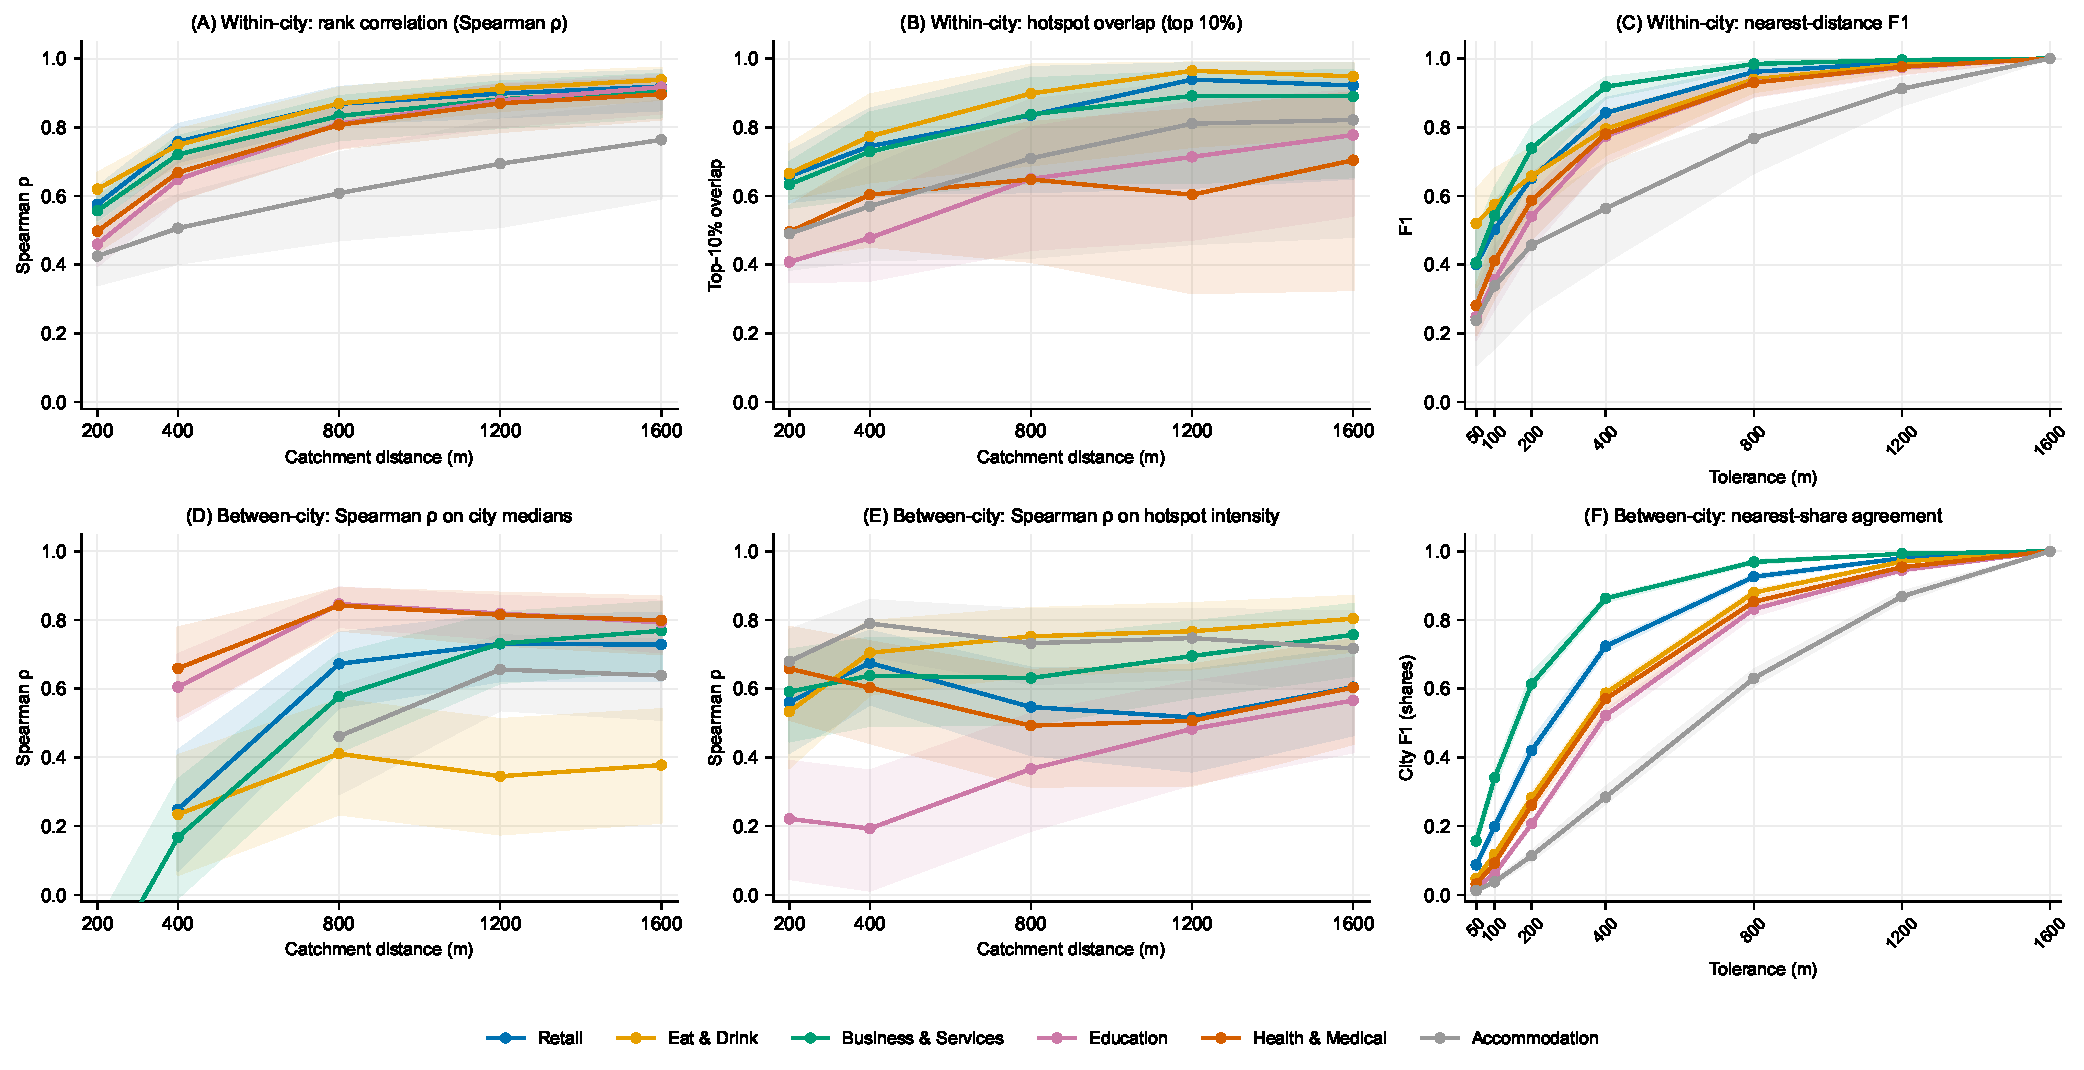
\includegraphics[width=\textwidth]{outputs/figures/fig_pointa_agreement_panels.pdf}
  \caption{\textbf{POI source-substitution agreement by category, task, and spatial scale.}
    \NRefCities{} reference cities. Top row (within-city): (A)~rank correlation (Spearman $\rho$), (B)~hotspot overlap, and (C)~nearest-within-tolerance F1; shaded bands show 95\% spatial block bootstrap CIs (distance-adaptive blocks, $B=200$). Bottom row (between-city): (D)~Spearman $\rho$ on city-level median counts, (E)~Spearman $\rho$ on city-level hotspot intensity, and (F)~harmonic-mean agreement of city-level nearest shares; shaded bands show 95\% city-level bootstrap CIs ($B=2{,}000$).
  }
  \label{fig:pointa_agreement_panels}
\end{figure}

\subsection{Per-city variability}
\label{sec:poi-supp-city-variability}

The main-text figures report median agreement across reference cities. Figure~\ref{fig:pointa_city_variability} shows the underlying per-city distributions at two representative catchment distances (400\,m and 800\,m). The strip plots confirm that the medians are not driven by a small number of outlier cities: at 800\,m most categories have tight distributions for rank correlation, with the bulk of cities exceeding 80\% concordance. Accommodation and Health \& Medical remain consistently the weakest categories with the widest spreads. Figure~\ref{fig:pointa_cross_city_scatter} complements this by plotting city-level median accessibility (log-transformed counts) from Overture against registry values at 800\,m; points falling below the identity line indicate systematic undercounting by Overture, particularly for Retail and Eat \& Drink.

\begin{figure}[p]
  \centering
  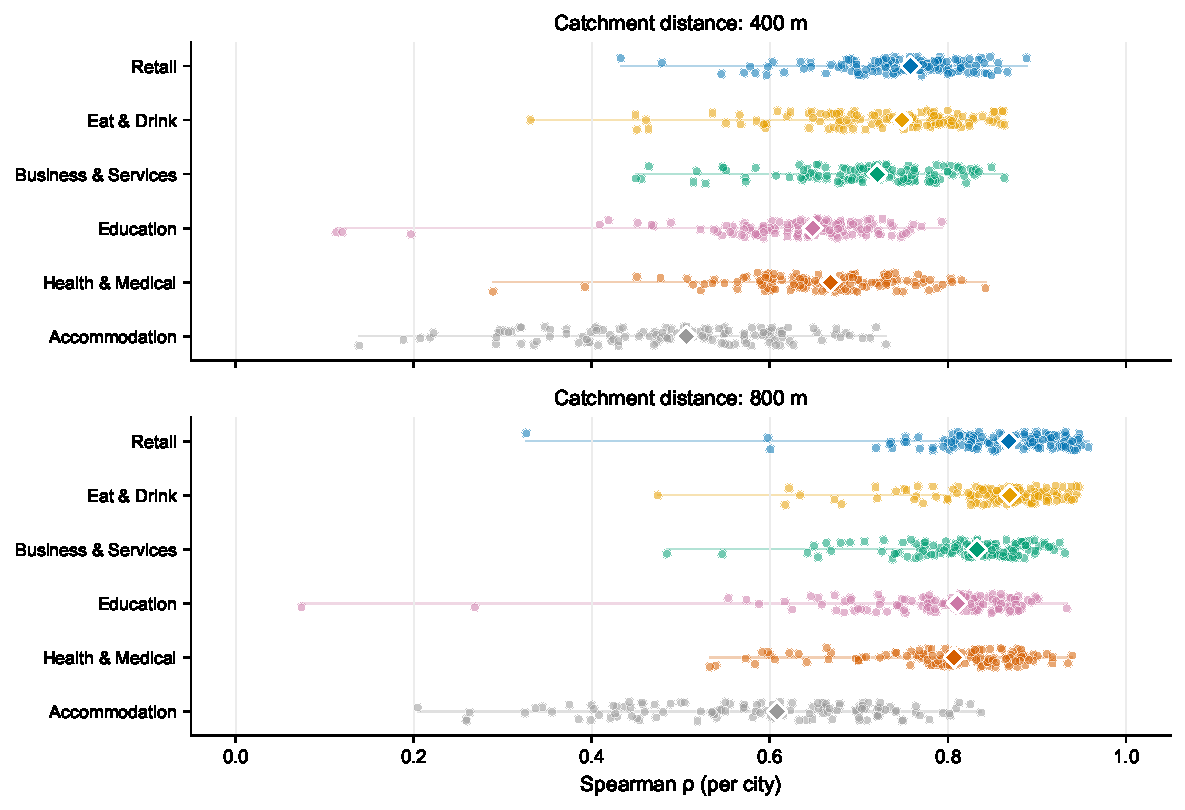
\includegraphics[width=0.88\textwidth]{outputs/figures/fig_pointa_city_variability.pdf}
  \caption{\textbf{Per-city rank correlation spread.}
    Distribution of Spearman $\rho$ (segment-level unweighted counts) across \NRefCities{} reference cities at 400\,m and 800\,m catchments. Points show individual cities; diamonds mark medians.
  }
  \label{fig:pointa_city_variability}

  \vspace{0.5em}

  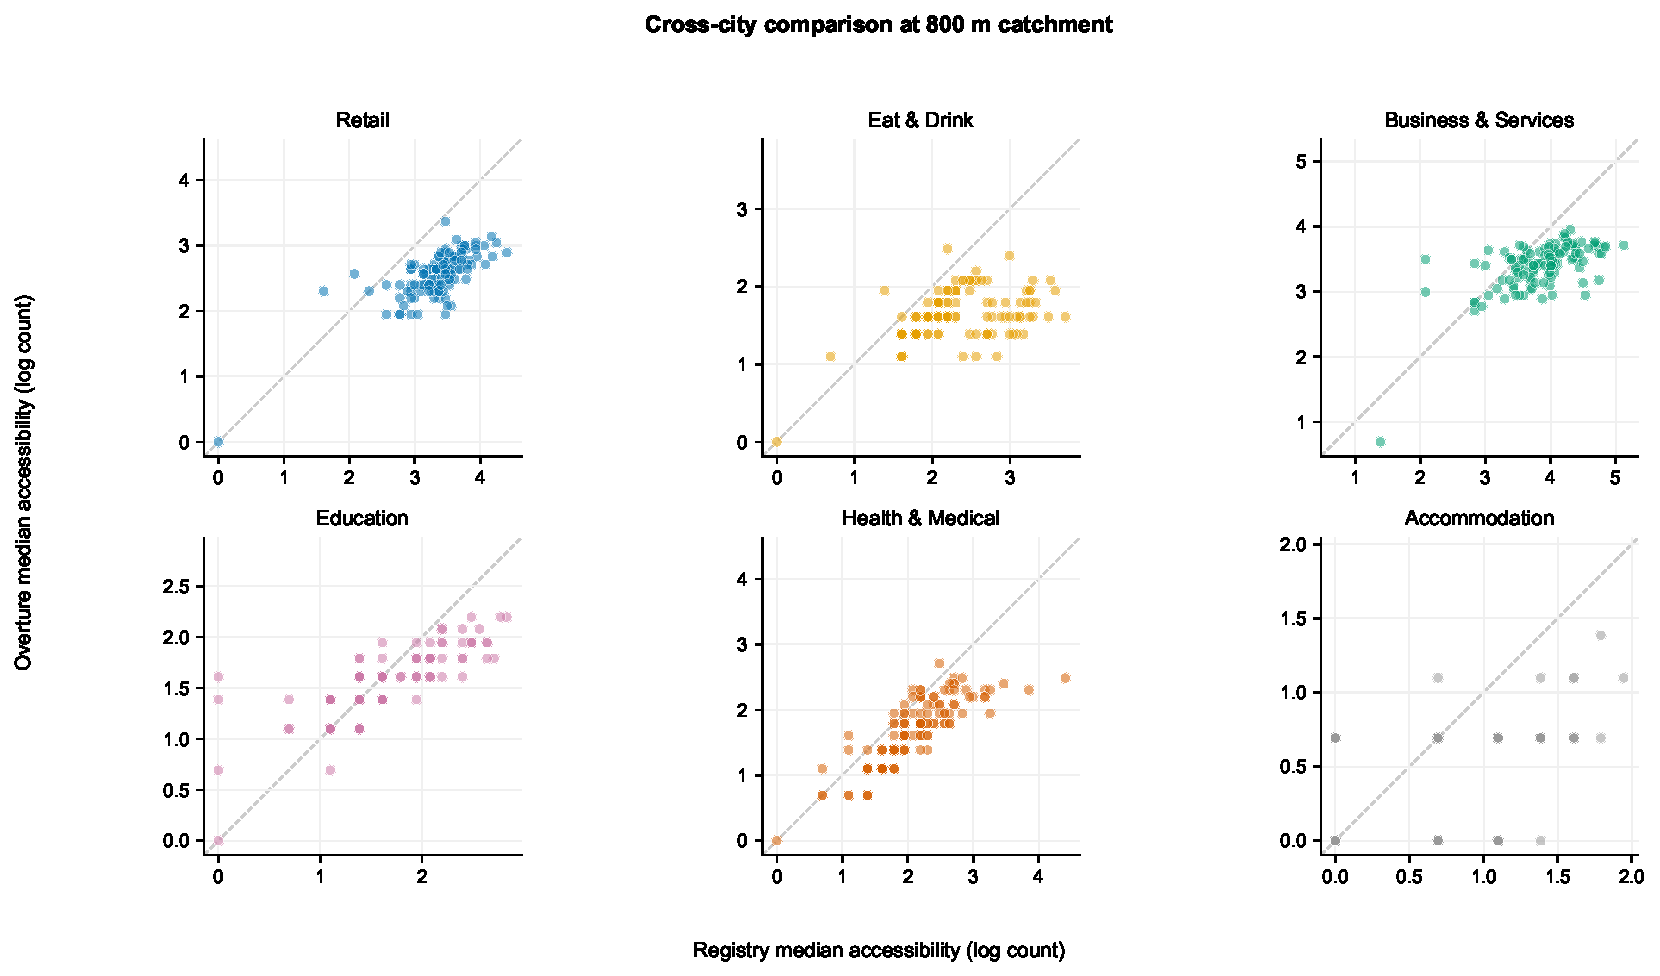
\includegraphics[width=0.88\textwidth]{outputs/figures/fig_pointa_cross_city_scatter.pdf}
  \captionof{figure}{\textbf{Cross-city comparison at 800\,m catchment.}
    Each point is one reference city. Axes show median log-transformed POI counts from registry and Overture sources; the dashed line marks identity. The predominance of points below the line indicates systematic undercounting by Overture, especially for Retail and Eat \& Drink.
  }
  \label{fig:pointa_cross_city_scatter}
\end{figure}

\subsection{Distance-weighted accessibility}
\label{sec:poi-supp-weighted}

The main-text results use unweighted POI counts (the number of establishments reachable within each catchment distance). An alternative is distance-weighted counts, where each POI's contribution decays with network distance, giving greater weight to nearer establishments. Figure~\ref{fig:pointa_agreement_panels_wt} reproduces the agreement curves of Figure~\ref{fig:pointa_agreement_panels} for distance-weighted counts, and Table~\ref{tab:pointa_minima_wt} the corresponding minimum agreement scales.

At the same catchment distance, weighted counts produce lower concordance than unweighted counts (typically 3--5 percentage points for rank correlation, 5--8 for hotspot overlap), because the gravity weighting amplifies the effect of small geocoding offsets between sources. However, the weighted measure at 800\,m still exceeds the unweighted measure at 400\,m across all categories, since the larger catchment more than compensates for the concordance lost to weighting. This is relevant for applications that prefer distance-weighted accessibility: reliable concordance is achievable at 800\,m or above. The nearest-distance columns are unchanged, as they do not involve count aggregation.

\begin{figure}[!htb]
  \centering
  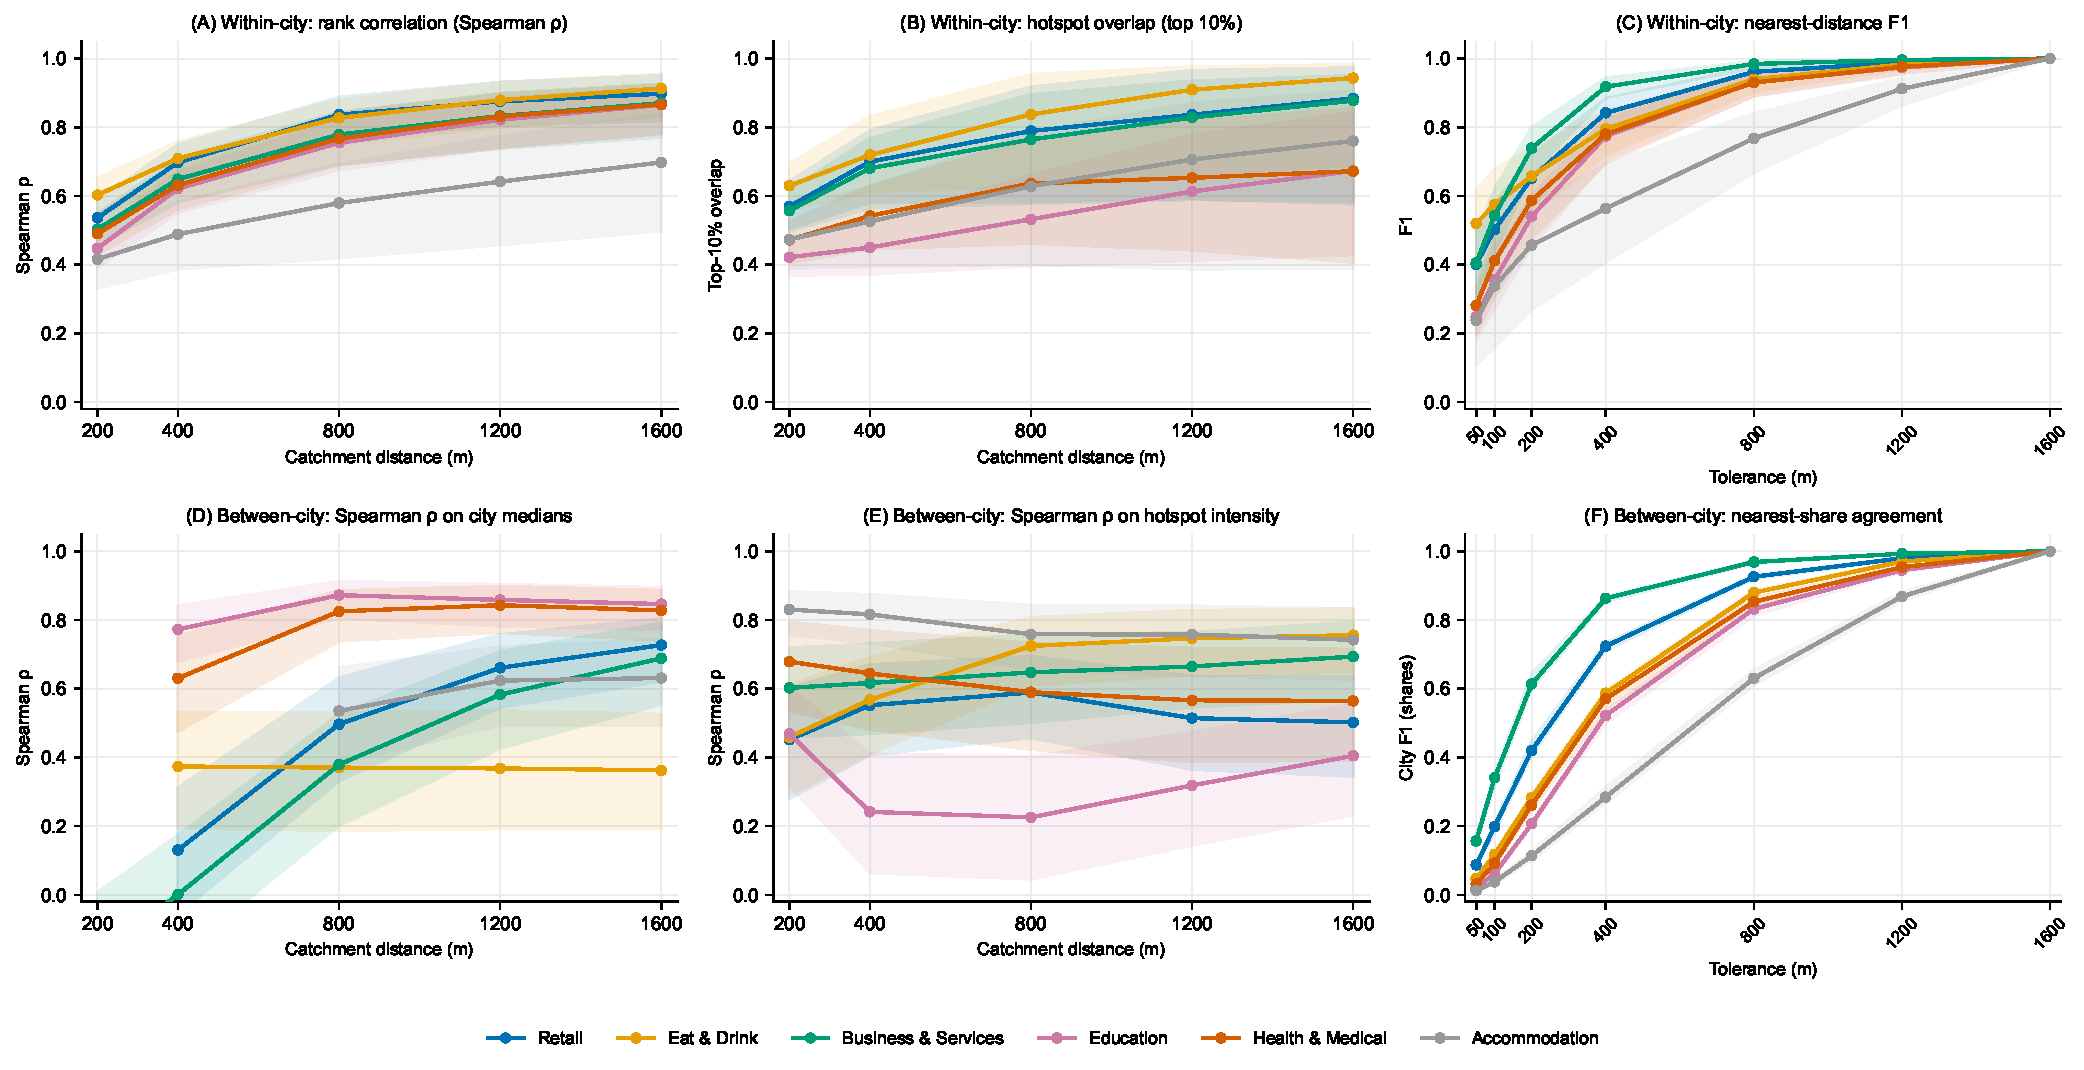
\includegraphics[width=\textwidth]{outputs/figures/fig_pointa_agreement_panels_wt.pdf}
  \caption{\textbf{POI source-substitution agreement for distance-weighted counts.}
    As Figure~\ref{fig:pointa_agreement_panels}, with count-based metrics computed on distance-weighted rather than unweighted POI counts; nearest-distance panels are unchanged by weighting.
  }
  \label{fig:pointa_agreement_panels_wt}
\end{figure}

\begin{table}[!htb]
  \centering
  \caption{Minimum spatial scale (metres) at which each category's median agreement reaches the concordance thresholds, for distance-weighted counts. As the corresponding unweighted-count table in the main text (Technical Validation); nearest-distance rows are unchanged by weighting.}
  \label{tab:pointa_minima_wt}
  \scriptsize
  \input{outputs/tables/table_pointa_minima_clean_wt}
\end{table}

\clearpage
\section{Building Footprint Source Composition and Metric Sensitivity}
\label{sec:bldg-supp}

This supplement documents the provenance composition of the Overture Maps building footprints used in SOAR-EU and quantifies its effect on derived morphometric indicators.

\subsection{Source classification}
\label{sec:bldg-supp-classification}

Each Overture building footprint carries a \texttt{sources} JSON array whose first element identifies the contributing dataset. We classify these into two groups: \emph{community-contributed} (OpenStreetMap, Esri Community Maps, national cadastral agencies) and \emph{ML-derived} (Microsoft ML Buildings, Google Open Buildings). Community-contributed footprints are digitised or imported from authoritative cadastral sources and generally preserve individual building boundaries; ML-derived footprints are segmented from satellite imagery and may merge adjacent buildings into single polygons or introduce unintended gaps between genuinely attached structures.

Across the \NCitiesTotal{} cities, the footprints draw on several source datasets: OpenStreetMap (dominant in most European cities), Esri Community Maps, Microsoft ML Buildings, and, in Spain, the Instituto Geogr\'{a}fico Nacional cadastre. Country-level aggregates reveal a clear geographic gradient (Table~\ref{tab:building_source_country}; Figure~\ref{fig:building_source_map}): the Netherlands, France, Switzerland, and Belgium are dominated by community sources, while Romania, Spain, Greece, and Bulgaria rely substantially on ML-derived footprints. The per-city ML fraction (Min and Max columns of Table~\ref{tab:building_source_country}) spans from zero in several cadastral-import cities to a large majority in the most ML-reliant. Per-city counts by dataset and country-level summaries are provided in the accompanying CSV files.

\begin{table}[!htb]
  \centering
  \caption{Building footprint source composition by country, sorted by ML-derived fraction (ascending). ML~(\%) is the proportion of footprints from ML-derived sources (primarily Microsoft ML Buildings); Min and Max show the per-city range within each country.}
  \label{tab:building_source_country}
  \scriptsize
  \begin{tabular}{@{}lrrrrr@{}}
  \toprule
  \textbf{Country} & \textbf{Cities} & \textbf{Buildings} & \textbf{ML (\%)} & \textbf{Min (\%)} & \textbf{Max (\%)} \\
  \midrule
  Netherlands & 43 & 6,209,242 & 1.6 & 0.0 & 20.6 \\
  Switzerland & 17 & 794,674 & 4.1 & 0.0 & 11.6 \\
  Luxembourg & 1 & 40,614 & 4.4 & 4.4 & 4.4 \\
  France & 73 & 10,245,743 & 4.5 & 0.0 & 15.2 \\
  Belgium & 16 & 2,627,084 & 5.2 & 1.0 & 16.2 \\
  Ireland & 5 & 769,998 & 5.4 & 3.3 & 8.4 \\
  Norway & 7 & 606,824 & 6.6 & 4.8 & 10.1 \\
  Finland & 6 & 367,553 & 7.8 & 6.2 & 13.5 \\
  Austria & 8 & 688,439 & 8.1 & 4.6 & 18.4 \\
  Denmark & 5 & 647,562 & 8.4 & 5.7 & 9.4 \\
  Estonia & 2 & 102,363 & 8.5 & 6.1 & 13.5 \\
  Germany & 99 & 11,601,375 & 8.8 & 0.1 & 35.7 \\
  Slovakia & 7 & 303,986 & 13.9 & 10.6 & 19.4 \\
  Slovenia & 2 & 98,624 & 15.3 & 13.4 & 19.0 \\
  Lithuania & 4 & 228,098 & 15.7 & 7.8 & 27.1 \\
  Latvia & 2 & 180,865 & 16.1 & 15.8 & 16.7 \\
  Czechia & 12 & 763,959 & 16.7 & 11.6 & 22.1 \\
  Italy & 88 & 4,246,128 & 17.4 & 3.0 & 81.0 \\
  Sweden & 17 & 793,793 & 18.5 & 0.7 & 50.7 \\
  Poland & 63 & 3,612,250 & 18.6 & 4.8 & 37.1 \\
  Croatia & 5 & 272,798 & 24.6 & 16.6 & 33.8 \\
  Hungary & 13 & 944,965 & 27.3 & 16.8 & 61.3 \\
  Portugal & 8 & 916,488 & 27.6 & 18.5 & 57.3 \\
  Bulgaria & 6 & 290,571 & 30.8 & 23.8 & 46.9 \\
  Greece & 8 & 871,146 & 31.3 & 7.5 & 94.9 \\
  Spain & 79 & 3,363,448 & 46.3 & 4.7 & 94.9 \\
  Romania & 29 & 1,319,339 & 48.0 & 23.6 & 86.1 \\
  Malta & 1 & 49,893 & 54.8 & 54.8 & 54.8 \\
  \bottomrule
\end{tabular}
\end{table}

\begin{figure}[!htb]
  \centering
  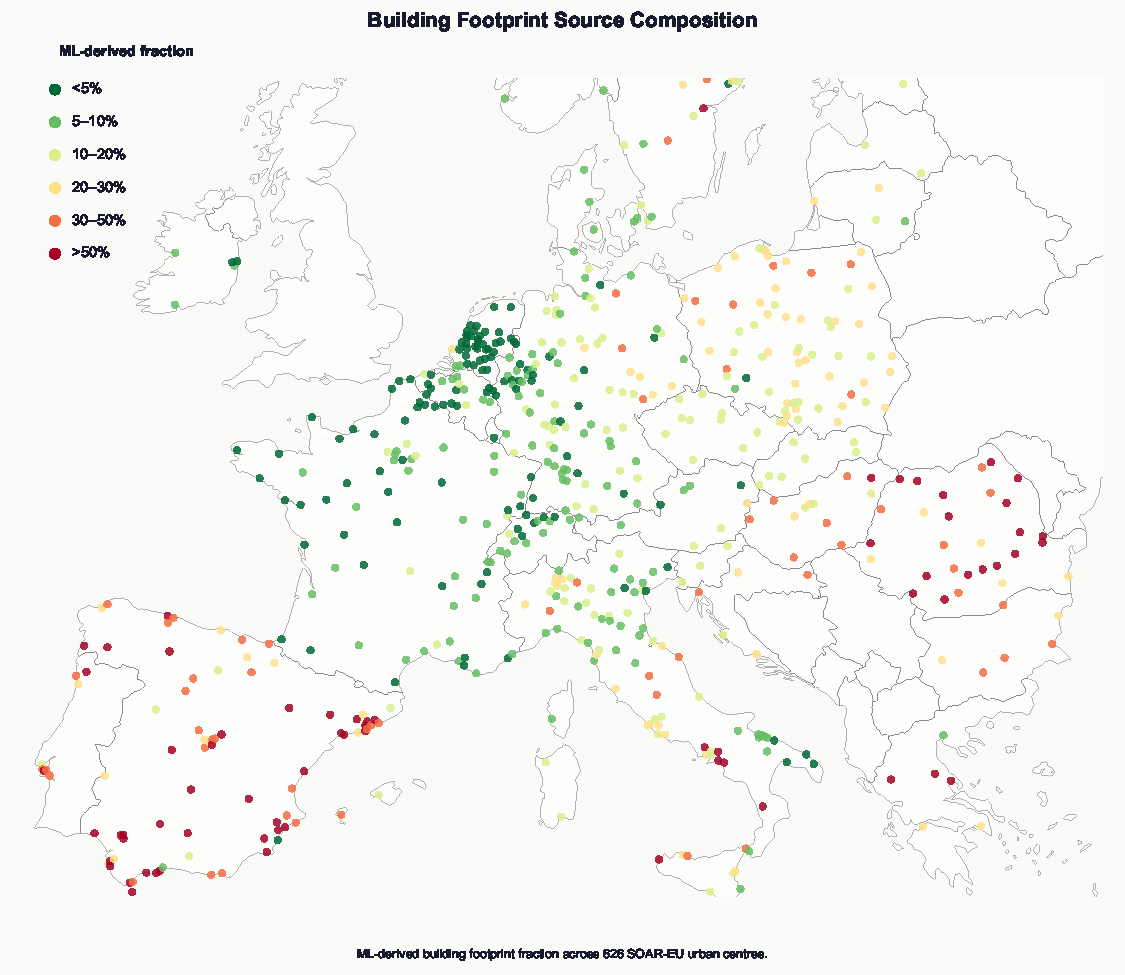
\includegraphics[width=\textwidth]{outputs/figures/fig_building_source_map.pdf}
  \caption{ML-derived building footprint fraction across the \NCitiesTotal{} SOAR-EU urban centres. Cities in western and northern Europe (France, Netherlands, Belgium, Germany) are dominated by community-contributed sources; cities in southern and eastern Europe (Romania, Spain, Greece, Bulgaria) rely more heavily on ML-derived footprints.}
  \label{fig:building_source_map}
\end{figure}

\subsection{Effect on morphometric indicators}
\label{sec:bldg-supp-sensitivity}

We test for source-driven bias at two levels.

\paragraph{Cross-city correlations.} For each morphometric indicator, we compute the Spearman correlation between each city's ML fraction and its median metric value across the \NCitiesTotal{} cities (Table~\ref{tab:building_metric_sensitivity}). Shared wall ratio shows the strongest negative association: cities with more ML-derived buildings have lower shared wall ratios. This cross-city correlation conflates two effects: a genuine morphological gradient (countries with higher ML fractions (Romania, Bulgaria, Greece) also have more freestanding housing stock) and a data artefact (ML-derived footprints underestimate shared walls due to polygon boundary gaps). The within-city test below isolates the artefact component. Perimeter, area, and volume are also positively associated, partly reflecting the tendency of ML segmentation to merge adjacent buildings into larger polygons and partly reflecting genuinely larger building footprints in lower-density settings. Fractal dimension and corner count show weaker but significant associations, while compactness, shape index, and orientation show no significant association with source composition.

\paragraph{Within-city comparisons.} To isolate the data artefact from genuine morphological differences between countries, we compare community and ML-derived buildings \emph{within the same city} using Mann--Whitney $U$ tests, restricted to cities containing both source types (Table~\ref{tab:building_metric_sensitivity}). Shared wall ratio shows a consistent within-city difference, significant in nearly all such cities: ML-derived buildings have lower shared wall ratios than community-contributed buildings in the same urban context, confirming a per-building artefact independent of cross-country morphological variation. Corner count and fractal dimension are also affected within cities, while compactness and shape index show small but widespread differences.

Block-level density metrics (GSI, FSI) show positive cross-city associations with ML fraction, FSI more strongly than GSI (Table~\ref{tab:building_metric_sensitivity}); as with the size metrics, these cross-city associations conflate a genuine morphological gradient (countries with higher ML fractions also tend towards denser building stock) with any source effect. Table~\ref{tab:building_metric_sensitivity} summarises all cross-city and within-city results.

\begin{table}[!htb]
  \centering
  \caption{Sensitivity of building morphometric indicators to data source composition. Cross-city $\rho$: Spearman correlation between city ML fraction and city median metric value, across all \NCitiesTotal{} cities. Within-city $r$: median rank-biserial correlation from Mann--Whitney $U$ tests comparing community and ML-derived buildings within each city, restricted to cities containing both source types. Significance: {*}{*}{*}\,$p < 0.001$, {*}{*}\,$p < 0.01$, {*}\,$p < 0.05$.}
  \label{tab:building_metric_sensitivity}
  \scriptsize
  \begin{tabular}{@{}lrrrl@{}}
  \toprule
  \textbf{Metric} & \textbf{Cross-city $\rho$} & \textbf{$p$} & \textbf{Within-city $r$} & \textbf{Sig.} \\
  \midrule
  Perimeter & +0.534 & $<$0.001 & --- & *** \\
  Shared Wall Ratio & -0.515 & $<$0.001 & -0.36 & *** \\
  Area & +0.513 & $<$0.001 & --- & *** \\
  Volume & +0.508 & $<$0.001 & --- & *** \\
  Shared Walls & -0.437 & $<$0.001 & --- & *** \\
  Block FSI & +0.372 & $<$0.001 & --- & *** \\
  Form Factor & -0.217 & $<$0.001 & --- & *** \\
  Fractal Dimension & -0.196 & $<$0.001 & -0.12 & *** \\
  Frontage Max & -0.178 & $<$0.001 & --- & *** \\
  Block GSI & +0.111 & 0.006 & --- & ** \\
  Corners & +0.098 & 0.015 & -0.26 & * \\
  Mean Height & +0.098 & 0.016 & --- & * \\
  Orientation & -0.060 & 0.136 & --- &  \\
  Compactness & +0.055 & 0.171 & +0.13 &  \\
  Shape Index & +0.055 & 0.171 & +0.13 &  \\
  \bottomrule
\end{tabular}
\end{table}

\subsection{Street-frontage ratio}
\label{sec:bldg-supp-frontage}

To provide a source-robust continuity measure, we compute a bilateral street-frontage ratio for each street segment. The computation proceeds as follows: (1)~buffer the street centreline by 35\,m to define a corridor (wide enough to capture building edges that address the street across a typical European front-garden or setback depth, narrow enough to exclude buildings on the next parallel street); (2)~identify all building edges whose midpoint falls inside the corridor and whose nearest street is this one (preventing cross-street contamination); (3)~classify each edge as left or right of the centreline using the local street tangent; (4)~per side, retain only edges within 5\,m of the closest edge, filtering out rear extensions and garages while preserving the primary facade line (5\,m is chosen to span typical facade step-ins and arcades without admitting rear-yard structures); (5)~project retained edges onto the centreline, merge overlapping intervals, and compute coverage as the fraction of street length covered (3\,m trimmed from each end as a junction guard, removing the short overlap where a corner property's facade would otherwise count towards both intersecting streets); (6)~the reported score (\texttt{frontage\_max}) is the maximum of the two sides. Per-side scores (\texttt{frontage\_left}, \texttt{frontage\_right}), their mean (\texttt{frontage\_avg}), and per-side edge counts (\texttt{frontage\_edges\_left}, \texttt{frontage\_edges\_right}) are also retained.

Unlike shared wall ratio, which requires exact topological contact between adjacent polygon boundaries, frontage ratio depends only on building \emph{presence} along the street edge. Whether two adjacent terraced houses are represented as separate touching polygons (community-digitised) or as a single merged polygon (ML-derived), the frontage coverage is the same. Across the \NCitiesTotal{} cities, the association between city-level ML fraction and median frontage ratio is substantially weaker than the corresponding shared-wall-ratio association (Table~\ref{tab:building_metric_sensitivity}). Because frontage is largely immune to the polygon-merging artefact that the within-city test identifies for shared wall ratio, this weaker residual association most likely reflects a predominantly genuine morphological gradient (countries with higher ML fractions also tend towards more freestanding housing) rather than a measurement artefact.


\begin{thebibliography}{2}

  \bibitem{sirene2026} INSEE. Base SIRENE des entreprises et de leurs \'{e}tablissements (SIREN, SIRET) [dataset]. \url{https://www.data.gouv.fr/en/datasets/base-sirene-des-entreprises-et-de-leurs-etablissements-siren-siret/} (2026). Open License 2.0 (Etalab).

  \bibitem{bag2026} Kadaster. BAG 2.0 Extract [dataset]. \url{https://www.kadaster.nl/zakelijk/producten/adressen-en-gebouwen/bag-2.0-extract} (2026). CC Public Domain Mark 1.0.

\end{thebibliography}

\end{document}
